\documentclass[fleqn, a4paper, 12pt, twoside]{article}

\newcounter{recitationcount} %creates a new counter for recitation numbers (must be executed before exsheets is loaded)
\newcommand\recitation{\refstepcounter{recitationcount}}

\usepackage[counter-within = recitationcount]{exsheets}
\usepackage{tasks}
\usepackage{amsmath, amssymb, amsthm} %standard AMS packages
\usepackage{esint} %integral signs
\usepackage{marginnote} %marginnotes
\usepackage{gensymb} %miscellaneous symbols
\usepackage{commath} %differential symbols
\usepackage{xcolor} %colours
\usepackage{cancel} %cancelling terms
\usepackage{siunitx} %formatting units
\usepackage{tikz, pgfplots} %diagrams
	\usetikzlibrary{calc, hobby, patterns, intersections, angles}
\usepackage{graphicx} %inserting graphics
\usepackage{hyperref} %hyperlinks
\usepackage{datetime} %date and time
\usepackage{ulem} %underline for \emph{}
\usepackage{xfrac, lmodern} %inline fractions
\usepackage{enumerate, enumitem} %numbered lists
\usepackage{float} %inserting floats
\usepackage[american voltages]{circuitikz} %circuit diagrams

\newcommand\numberthis{\addtocounter{equation}{1}\tag{\theequation}} %adds numbers to specific equations in non-numbered list of equations

\newcommand{\AxisRotator}[1][rotate=0]{
	\tikz [x=0.25cm,y=0.60cm,line width=.2ex,-stealth,#1] \draw (0,0) arc (-150:150:1 and 1);%
} %rotation symbols on axes

\theoremstyle{definition}
\newtheorem{example}{Example}
\newtheorem{definition}{Definition}

\theoremstyle{theorem}
\newtheorem{theorem}{Theorem}

\newcommand{\curl}{\mathrm{curl\,}}

\makeatletter
\@addtoreset{section}{part} %resets section numbers in new part
\makeatother

\makeatletter
% Helper macros
\def\tikz@lib@angle@def@coord#1{%
  \ifx(#1\relax
    \coordinate(tikz@lib@angle@tmp)at#1;%
  \else
    \coordinate(tikz@lib@angle@tmp)at(#1);%
  \fi
}
\def\tikz@lib@angle@coord#1{%
  \pgf@process{% 
    \ifx(#1\relax
      \tikz@scan@one@point\@firstofone#1\relax
    \else
      \pgfpointanchor{#1}{center}%
    \fi
  }%
}
% Patching
\patchcmd\tikz@lib@angle@background{#2}{tikz@lib@angle@tmp}{}{%
  \errmessage{Cannot patch \string\tikz@lib@angle@background}%
}
\patchcmd\tikz@lib@angle@foreground{#2}{tikz@lib@angle@tmp}{}{%
  \errmessage{Cannot patch \string\tikz@lib@angle@foreground}%
}
\pretocmd\tikz@lib@angle@background{\tikz@lib@angle@def@coord{#2}}{}{%
  \errmessage{Cannot prepend \string\tikz@lib@angle@background}%
}
\pretocmd\tikz@lib@angle@foreground{\tikz@lib@angle@def@coord{#2}}{}{%
  \errmessage{Cannot prepend \string\tikz@lib@angle@foreground}%
}
\patchcmd\tikz@lib@angle@parse{%
  \pgf@process{\pgfpointanchor{#2}{center}}%
}{%
  \tikz@lib@angle@coord{#2}%
}{}{%
  \errmessage{Cannot patch \string\tikz@lib@angle@parse}%
}
\patchcmd\tikz@lib@angle@parse{%
  \pgf@process{\pgfpointanchor{#1}{center}}%
}{%
  \tikz@lib@angle@coord{#1}%
}{}{%
  \errmessage{Cannot patch \string\tikz@lib@angle@parse}%
}
\patchcmd\tikz@lib@angle@parse{%
  \pgf@process{\pgfpointanchor{#3}{center}}%
}{%
  \tikz@lib@angle@coord{#3}%
}{}{%
  \errmessage{Cannot patch \string\tikz@lib@angle@parse}%
}
% Better support for the comma in the value for angle:
\tikzset{
  pics/angle/.style = {
    setup code  = {\tikz@lib@angle@parse#1\pgf@stop},
    background code = {\tikz@lib@angle@background#1\pgf@stop},
    foreground code = {\tikz@lib@angle@foreground#1\pgf@stop},
  },
}
\makeatother

\newcommand\blfootnote[1]{%
	\begingroup
	\renewcommand\thefootnote{}\footnote{#1}%
	\addtocounter{footnote}{-1}%
	\endgroup
}

\RenewQuSolPair{question}[name=Recitation \therecitationcount\ -- Exercise]{solution}[name=Recitation \therecitationcount\ -- Solution]

\SetupExSheets{solution/print = true, totoc = true} %prints all solutions by default

%opening
\title{Physics 2 : Recitations}
\author{Aakash Jog}
\date{2014-15}

\begin{document}

\maketitle
%\setlength{\mathindent}{0pt}

\blfootnote
{	
	\begin{figure}[H]
		\includegraphics[height = 12pt]{cc.eps}
		\includegraphics[height = 12pt]{by.eps}
		\includegraphics[height = 12pt]{nc.eps}
		\includegraphics[height = 12pt]{sa.eps}
	\end{figure}
	This work is licensed under the Creative Commons Attribution-NonCommercial-ShareAlike 4.0 International License. To view a copy of this license, visit \url{http://creativecommons.org/licenses/by-nc-sa/4.0/}.
} %CC-BY-NC-SA licencse

\tableofcontents

\newpage
\section{Instructor Information}

\textbf{Dr. Richard Spitzberg}\\
~\\
Office: Ma Aabadot 119\\
E-mail: rms9999@gmail.com\\

\newpage

\part{Electrostatics}

\section{Gravitation and Electromagnetism}

\begin{tabular}{l l}
	Gravitation & Electromagnetism\\
		$F_G = G \dfrac{m_1 m_2}{r^2}$ & $F_E = k \dfrac{q_1 q_2}{r^2}$\\
		$G = 6.7 \times 10^{11} \si{\newton\metre\squared\per\kg\squared}$ & $8.99 \times 10^9 \si{\newton\metre\squared\per\coulomb\squared}$\\
\end{tabular}

\section{Coulomb's Law}

\recitation

\begin{question}
	Four identical charges $q$ are placed in the corners of a square of length $a$. A fifth charge $Q$ is free to move along the straight line perpendicular to the square plane and passing through its centre. When the charge $Q$ is in the same plane as the other charges, all the forces in the system cancel out.
	\begin{enumerate}
		\item Calculate $Q$ for a given $q$ and $a$.
		\item Find the force $\overrightarrow{F(z)}$ acting on the charge $Q$ when it is at height $z$ above the square.
	\end{enumerate}
\end{question}

\begin{solution}[print]
	\begin{figure}[H]
		\begin{tikzpicture}
			\def\a{4};
			
			\draw (-\a/2,-\a/2) rectangle (\a/2,\a/2);
			
			\filldraw ({-\a/2},{-\a/2}) circle [radius = 2pt] node [below left] {$q$};
			\filldraw ({-\a/2},{\a/2}) circle [radius = 2pt] node [above left] {$q$};
			\filldraw ({\a/2},{\a/2}) circle [radius = 2pt] node [above right] {$q$};
			\filldraw ({\a/2},{-\a/2}) circle [radius = 2pt] node [below right] {$q$};
			
			\filldraw (0,0) circle [radius = 2pt] node [left] {$Q$};
		\end{tikzpicture}
	\end{figure}
	Consider $q$ on the top right corner of the square. The total force acting on it is 0. Therefore
	\begin{align*}
		0 &= \dfrac{k q^2}{a^2} \cos \dfrac{\pi}{4} + \dfrac{k q^2}{a^2} \cos \dfrac{\pi}{4} + \dfrac{k q^2}{2 a^2} + \dfrac{2 k Q q}{a^2}\\
		\therefore Q &= - \dfrac{1 + 2 \sqrt{2}}{4} q
	\end{align*}
	~\\
	If $Q$ is at a height $z$ from the plane, the distance between each $q$ and $Q$ is
	\begin{align*}
		r &= \sqrt{z^2 + \left( \dfrac{a}{\sqrt{2}} \right)^2}
	\end{align*}
	Therefore the force of each $q$ on $Q$ is $\dfrac{k Q q}{r^2}$.\\
	Due to symmetry, the components of the forces in the $z$ direction will add up, and all other components will cancel out.\\
	Let the angle between the $z$ direction and the line joining $q$ and $Q$ be $\varphi$.\\
	Therefore, the net force is 
	\begin{align*}
		F &= 4 \dfrac{k Q q}{r^2} \cos \varphi\\
		&= 4 \dfrac{k Q q}{r^2} \dfrac{z}{r}\\
		&= 4 \dfrac{k Q q}{z^2 \left( 1 + \dfrac{a^2}{2 z^2} \right)^{\sfrac{3}{2}}}
	\end{align*}
\end{solution}

\begin{question}
	\begin{enumerate}
		\item A wire of length 3 \si{metre} is charged with 2 \si{\coulomb\per\metre}. What is the wire's total charge?
	\end{enumerate}
\end{question}

\begin{solution}[print]
	\begin{align*}
		\lambda &= \dfrac{Q}{L}\\
		\therefore Q &= L \lambda\\
		&= 6 \si{\coulomb}
	\end{align*}
\end{solution}

\begin{question}
	A wire of length $L$ has the following charge distribution: $\lambda = \lambda_0 \cos \dfrac{\pi x}{L}$, where $x$ is the distance from the wire's edge. What is the wire's total charge?
\end{question}

\begin{solution}[print]
	\begin{align*}
		\lambda &= \dod{q}{x}\\
		\therefore \dod{q}{x} &= \lambda_0 \cos \dfrac{\pi x}{L}\\
		\therefore q &= \int\limits_{0}^{L} \lambda_0 \cos \dfrac{\pi x}{L} \dif x\\
		&= 0
	\end{align*}
\end{solution}

\begin{question}
	A hollow sphere of radius $R$ is uniformly charged with a charge $Q$. Calculate the charge distribution on the surface of the sphere.
\end{question}

\begin{solution}[print]
	\begin{align*}
		\sigma &= \dfrac{Q}{A}\\
		&= \dfrac{Q}{4 \pi R^2}
	\end{align*}
\end{solution}

\begin{question}
	A straight thin wire is uniformly charged with distribution $\lambda$. A charge $q$ is positioned at distance $y_1$ beneath the wire and $r$ away form it.
	\begin{enumerate}
		\item Find the force acting on the charge $q$.
		\item Show that when the charge is positioned in front of the centre of the wire the $\hat{y}$ component of the force is cancelled.
		\item Calculate the force an infinite straight wire will exert on the charge $q$.
	\end{enumerate}
\end{question}

\begin{solution}[print]
	\begin{figure}[H]
		\begin{tikzpicture}
			\def\L{3};
			\def\y{2};
			\def\r{2};
			\def\Y{1};
			
			\def\xMAX{\L + \Y + 1};
			\def\yMAX{\r + 1};
			
			\begin{scope}[gray, -stealth]
				\draw (0,0) -- (\xMAX,0) node [right] {$y$};
				\draw (0,0) -- (0,\yMAX) node [above] {$z$};
			\end{scope}
			
			\draw [ultra thick, red] (0,0) -- (\L,0);
			
			\begin{scope}[|-stealth, yshift = -10]
				\draw (\L,0) -- ++(\Y,0) node [below] {$y_1$};
				\draw (0,0) -- (\y,0) node [below] {$y$};
				\draw [yshift = -10] (0,0) -- (\L,0) node [below] {$L$};
			\end{scope}
			
			\filldraw ({\L + \Y}, \r) circle [radius = 2pt] node [left] {$q$};
			
			\begin{scope}[dashed]
				\draw ({\L + \Y},0) -- ({\L + \Y}, \r) node [midway, right] {$r$};
				\draw (\y,0) -- ({\L + \Y}, \r) node [midway, above left] {$R$};
			\end{scope}
		\end{tikzpicture}
	\end{figure}
	Consider an elemental charge $\dif Q$ of length $\dif y$, at distance $y$ as shown. Let the angle between the line joining $\dif Q$ and $q$ and the $y$ direction be $\theta$.
	\begin{align*}
		F_y &= F \cos \theta\\
		F_z &= F \sin \theta\\
	\end{align*}
	Let
	\begin{align*}
		a &= L + y_1\\
		\therefore R &= \sqrt{r^2 + (a - y)^2}
	\end{align*}
	Therefore,
	\begin{align*}
		\cos \theta &= \dfrac{a - y}{R}\\
		\sin \theta &= \dfrac{r}{R}
	\end{align*}
	Therefore,
	\begin{align*}
		F_y &= k q \int\limits_{0}^{L} \dfrac{\lambda \dif y}{R^2} \dfrac{(a - y)}{R}\\
		&= k q \lambda \int\limits_{0}^{L} \dfrac{\dif y (a - y)}{\left( (a - y)^2 + r^2 \right)^{\sfrac{3}{2}}}\\
		&= k q \lambda \left( \dfrac{1}{\sqrt{{y_1}^2 + r^2}} - \dfrac{1}{\sqrt{a^2 + r^2}} \right)
	\end{align*}
	\begin{align*}
		F_z &= k q \int\limits_{0}^{L} \dfrac{\lambda \dif y}{R^2} \dfrac{r}{R}\\
		&= k q \lambda \int\limits_{0}^{L} \dfrac{r \dif y}{\left( (a - y)^2 + r^2 \right)^{\sfrac{3}{2}}}\\
		&= \dfrac{k q \lambda}{r} \left( \dfrac{a}{\sqrt{r^2 + a^2}} - \dfrac{y_1}{\sqrt{r^2 + {y_1}^2}} \right)
	\end{align*}
	~\\
	When the charge is positioned above the centre of the wire,
	\begin{align*}
		y_1 &= -\dfrac{L}{2}\\
		\therefore a &= \dfrac{L}{2}
	\end{align*}
	Therefore,
	\begin{align*}
		F_y &= k q \lambda \left( \dfrac{1}{\sqrt{{y_1}^2 + r^2}} - \dfrac{1}{\sqrt{a^2 + r^2}} \right)\\
		&= k q \lambda \left( \dfrac{1}{\sqrt{{-\dfrac{L}{2}}^2 + r^2}} - \dfrac{1}{\sqrt{{\dfrac{L}{2}}^2 + r^2}} \right)\\
		&= 0
	\end{align*}
	\begin{align*}
		F_z &= \dfrac{k q \lambda}{r} \left( \dfrac{a}{\sqrt{r^2 + a^2}} - \dfrac{y_1}{\sqrt{r^2 + {y_1}^2}} \right)\\
		&= \dfrac{k q \lambda}{r} \left( \dfrac{\dfrac{L}{2}}{\sqrt{r^2 + {\dfrac{L}{2}}^2}} - \dfrac{-\dfrac{L}{2}}{\sqrt{r^2 + {-\dfrac{L}{2}}^2}} \right)\\
		&= \dfrac{k q \lambda}{r} \left( \dfrac{L}{\sqrt{r^2 + {\dfrac{L}{2}}^2}} \right)\\
		&= \dfrac{k q \lambda}{r} \left( \dfrac{1}{\sqrt{\dfrac{1}{4} + \left( \dfrac{r}{L} \right)^2}} \right)
	\end{align*}
	~\\
	If the line is infinite, $L \to \infty$. Therefore
	\begin{align*}
		F_z &= \dfrac{k q \lambda}{r} \left( \dfrac{1}{\sqrt{\dfrac{1}{4} + \left( \dfrac{r}{L} \right)^2}} \right)\\
		&= \dfrac{2 k q \lambda}{r} 
	\end{align*}
\end{solution}

\section{Gauss' Law}

\recitation
\setcounter{question}{1}

\begin{question}
	A ball of radius $a$ is charged with distribution $\rho$ = $\rho_0 \dfrac{r}{a}$. Find the electric field everywhere.
\end{question}

\begin{solution}
	Consider a spherical Gaussian surface of radius $r$.\\
	If $r \leq a$, the charge in the interior of the Gaussian surface is
	\begin{align*}
		q(r) &= \int\limits_{0}^{r} \dfrac{\rho_0 r}{a} \cdot 4 \pi r^2 \dif r\\
		&= \dfrac{\rho_0}{a} \pi r^4
	\end{align*}
	Therefore, by Gauss' Law,
	\begin{align*}
		E \cdot 4 \pi r^2 &= \dfrac{q(r)}{\varepsilon_0}\\
		\therefore E &= \dfrac{\rho_0 \pi r^4}{4 \pi a r^2}\\
		&= \dfrac{\rho_0 r^2}{4 a \varepsilon_0}
	\end{align*}
	If $r \geq a$, the entire ball of charge is in the interior of the Gaussian surface.\\
	Therefore,
	\begin{align*}
		Q &= q(a)\\
		&= \dfrac{\rho_0}{a} \cdot \pi a^4\\
		&= \rho_0 \pi a^3
	\end{align*}
	Therefore, by Gauss' Law,
	\begin{align*}
		E \cdot 4 \pi r^2 &= \dfrac{Q}{\varepsilon_0}\\
		\therefore E &= \dfrac{Q}{4 \pi r^2 \varepsilon_0}\\
		&= \dfrac{\rho_0 a^3}{4 r^2 \varepsilon_0}
	\end{align*}
	~\\
	Therefore,
	\begin{align*}
		E &=
			\begin{cases}
				\dfrac{\rho_0 r^2}{4 a \varepsilon_0} &;\quad r \leq a\\
				\dfrac{\rho_0 a^3}{4 r^2 \varepsilon} &;\quad r \geq a\\
			\end{cases}
	\end{align*}
\end{solution}

\begin{question}
	An infinitely long cylinder of radius $a$ is charged with distribution $\rho = \rho_0 \dfrac{r}{a}$. Find the electric field everywhere.
\end{question}

\begin{solution}
	Consider a infinite cylindrical Gaussian surface with radius $r$.\\
	If $r \leq a$, the charge in the interior of the Gaussian surface is
	\begin{align*}
		q(r) &= \int\limits_{0}^{r} \dfrac{\rho_0 r}{a} \pi r^2 \dif r\\
		&= \dfrac{2 \pi \rho_0 L r^3}{3 a}
	\end{align*}
	Therefore, by Gauss' Law,
	\begin{align*}
		E \cdot 2 \pi r L &= \dfrac{2 \pi \rho_0 L r^3}{3 a \varepsilon_0}\\
		\therefore E &= \dfrac{\rho_0 r^2}{3 a \varepsilon_0}
	\end{align*}
	If $r \geq a$, the entire cylinder of charge is in the interior of the Gaussian surface.\\
	Therefore,
	\begin{align*}
		Q &= q(a)\\
		&= \dfrac{2 \pi \rho_0 L a^3}{3 a}\\
		&= \dfrac{2 \pi \rho_0 L a^2}{3}
	\end{align*}
	Therefore, by Gauss' Law,
	\begin{align*}
		E \cdot 2 \pi r L &= \dfrac{2 \pi \rho_0 L a^2}{3 \varepsilon_0}\\
		\therefore E &= \dfrac{\rho_0 a^2}{3 \varepsilon_0 r}
	\end{align*}
	~\\
	Therefore,
	\begin{align*}
		E &= 
			\begin{cases}
				\dfrac{\rho_0 r^2}{3 a \varepsilon_0} &;\quad r \leq a\\
				\dfrac{\rho_0 a^2}{3 \varepsilon_0 r} &; \quad r \geq a\\
			\end{cases}
	\end{align*}
\end{solution}

\begin{question}
	Find the electric field due to a thin infinite plane of uniform charge distribution $\sigma$.
\end{question}

\begin{solution}
	Consider a cylindrical Gaussian surface, with ends of area $A$, as shown.
	\begin{figure}[H]
		\begin{tikzpicture}
			\def\h{2};
			\def\r{1};
			\def\L{5};
			
			\draw [blue] ({-\L/2},0) -- ({\L/2},0) node [right] {$\sigma$};
			
			\begin{scope}[red]
				\draw (0,{-\h/2}) circle [x radius = \r, y radius = 0.4*\r];
				\draw (0,{\h/2}) circle [x radius = \r, y radius = 0.4*\r];
				
				\draw ({-\r},{-\h/2}) -- ({-\r},{\h/2});
				\draw ({\r},{-\h/2}) -- ({\r},{\h/2});
			\end{scope}
		\end{tikzpicture}
	\end{figure}
	The charge in the interior of the surface is
	\begin{align*}
		\dif q &= A \sigma
	\end{align*}
	Therefore, by Gauss' Law,
	\begin{align*}
		E_1 \cdot A_1 + E_2 \cdot A_2 &= \dfrac{A \sigma}{\varepsilon_0}\\
		\therefore 2 E A &= \dfrac{A \sigma}{\varepsilon_0}\\
		\therefore E &= \dfrac{\sigma}{2 \varepsilon_0}
	\end{align*}
\end{solution}

\recitation

\section{Electric Potential}

\setcounter{question}{1}

\begin{question}
	A system of four charges is constructed as shown.
	\begin{figure}[H]
		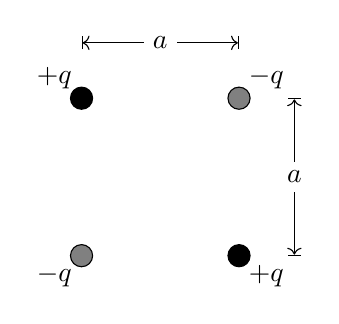
\begin{tikzpicture}
			\def\a{2};
			
			\filldraw [fill = gray]
				({\a/2},{\a/2}) circle (4pt) node [above right] {$-q$}
				({-\a/2},{-\a/2}) circle (4pt) node [below left] {$-q$};
				
			\filldraw [fill = black]
				({-\a/2},{\a/2}) circle (4pt) node [above left] {$+q$}
				({\a/2},{-\a/2}) circle (4pt) node [below right] {$+q$};
				
			\begin{scope}[|<->|]
				\draw [yshift = 20] ({-\a/2},{\a/2}) -- ({\a/2},{\a/2}) node [midway, fill = white] {$a$};
				\draw [xshift = 20] ({\a/2},{-\a/2}) -- ({\a/2},{\a/2}) node [midway, fill = white] {$a$};
			\end{scope}
		\end{tikzpicture}
	\end{figure}
	\begin{tasks}
		\task Calculate the work needed to build this system.
		\task What is the potential in the centre of the system?
		\task Calculate the potential in each of the corners (calculate as if there is no charge in the corner you are calculating for).
	\end{tasks}
\end{question}

\begin{solution}
	\begin{tasks}
		\task
			Let the positions of the charges be A, B, C, D.
			\begin{figure}[H]
				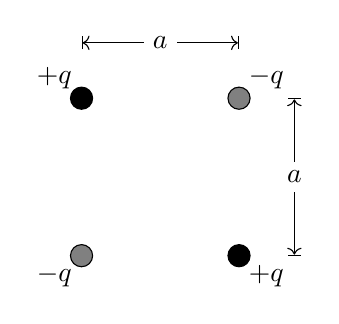
\begin{tikzpicture}
					\def\a{2};
					
					\filldraw [fill = gray]
						({\a/2},{\a/2}) circle (4pt) node [above right] {$-q$}
						({-\a/2},{-\a/2}) circle (4pt) node [below left] {$-q$};
					
					\filldraw [fill = black]
						({-\a/2},{\a/2}) circle (4pt) node [above left] {$+q$}
						({\a/2},{-\a/2}) circle (4pt) node [below right] {$+q$};
					
					\begin{scope}[|<->|]
						\draw [yshift = 20] ({-\a/2},{\a/2}) -- ({\a/2},{\a/2}) node [midway, fill = white] {$a$};
						\draw [xshift = 20] ({\a/2},{-\a/2}) -- ({\a/2},{\a/2}) node [midway, fill = white] {$a$};
					\end{scope}
				\end{tikzpicture}
			\end{figure}
			The work done to bring the first charge from infinity to A is
			\begin{align*}
				W_{\textnormal{A}} &= 0
			\end{align*}
			The work done to bring the first charge from infinity to B is
			\begin{align*}
				W_{\textnormal{B}} &= \dfrac{1}{4 \pi \varepsilon_0} \dfrac{q^2}{a \sqrt{2}}
			\end{align*}
			Similarly for the other two charges.\\
			Therefore,
			\begin{align*}
				W &= 0 + \dfrac{q^2}{4 \sqrt{2} \pi \varepsilon_0} + \dfrac{-2q^2}{4 \pi \varepsilon_0 a} + \left( \dfrac{-2q^2}{4 \pi \varepsilon_0 a} + \dfrac{q^2}{4 \sqrt{2} \pi \varepsilon_0} \right)\\
				&= \dfrac{q^2}{2 \sqrt{2} \pi \varepsilon_0} - \dfrac{q^2}{\pi \varepsilon_0 a}
			\end{align*}
		\task
			\begin{align*}
				V_{\textnormal{centre}} &= V_{q} + V_{q} + V_{-q} + V_{-q}\\
				&= \dfrac{q}{4 \pi \varepsilon_0 \left( \dfrac{a}{\sqrt{2}} \right)} + \dfrac{q}{4 \pi \varepsilon_0 \left( \dfrac{a}{\sqrt{2}} \right)} - \dfrac{q}{4 \pi \varepsilon_0 \left( \dfrac{a}{\sqrt{2}} \right)} - \dfrac{q}{4 \pi \varepsilon_0 \left( \dfrac{a}{\sqrt{2}} \right)}\\
				&= 0
			\end{align*}
		\task
			\begin{align*}
				V_{\textnormal{A}} &= \dfrac{1}{4 \pi \varepsilon_0} \dfrac{-q}{a} + \dfrac{1}{4 \pi \varepsilon_0} \dfrac{-q}{a} + \dfrac{1}{4 \pi \varepsilon_0} \dfrac{q}{\sqrt{2} a}\\
				V_{\textnormal{B}} &= \dfrac{1}{4 \pi \varepsilon_0} \dfrac{-q}{a} + \dfrac{1}{4 \pi \varepsilon_0} \dfrac{-q}{a} + \dfrac{1}{4 \pi \varepsilon_0} \dfrac{q}{\sqrt{2} a}\\
				V_{\textnormal{C}} &= \dfrac{1}{4 \pi \varepsilon_0} \dfrac{q}{a} + \dfrac{1}{4 \pi \varepsilon_0} \dfrac{q}{a} + \dfrac{1}{4 \pi \varepsilon_0} \dfrac{-q}{\sqrt{2} a}\\
				V_{\textnormal{D}} &= \dfrac{1}{4 \pi \varepsilon_0} \dfrac{q}{a} + \dfrac{1}{4 \pi \varepsilon_0} \dfrac{q}{a} + \dfrac{1}{4 \pi \varepsilon_0} \dfrac{-q}{\sqrt{2} a}
			\end{align*}
	\end{tasks}
\end{solution}

\begin{question}
	A ring of radius $R$ is charged with total charge $Q$.
	\begin{tasks}
		\task Calculate the electric field in the centre of the ring.
		\task Calculate the potential in the centre of the ring by integrating the contributions of the infinitesimal charge elements of the ring.
	\end{tasks}
\end{question}

\begin{solution}
	\begin{tasks}
		\task
			Due to the symmetry of the ring, the field due to every elemental charge $\dif q$ will be cancelled out by the field due to a elemental charge diametrically opposite to $\dif q$.\\
			Therefore, 
			\begin{align*}
				\overrightarrow{E} &= 0
			\end{align*}
		\task
			\begin{align*}
				\dif V &= \dfrac{\dif q}{4 \pi \varepsilon_0 R}\\
				\therefore V &= \dfrac{Q}{4 \pi \varepsilon_0 R}
			\end{align*}
	\end{tasks}
\end{solution}

\begin{question}
	Calculate the potential resulting from a ball charged with constant volume distribution $\rho$. Use the expression
	\begin{equation*}
		\varphi(r_2) - \varphi(r_1) = - \int\limits_{r_1}^{r_2} E(r) \dif r
	\end{equation*}
	Repeat the calculation twice:
	\begin{tasks}
		\task Set $\varphi(r = R) = 0$
		\task Set $\varphi(r = \infty) = 0$
	\end{tasks}
\end{question}

\begin{solution}
	\begin{tasks}
		\task
			Let $\varphi(r = \infty) = 0$.\\
			~\\
			If $r > R$,
			\begin{align*}
				E &= -\dod{\varphi}{r}\\
				\therefore -\dod{\varphi}{r} &= \dfrac{Q}{4 \pi \varepsilon_0 r^2}\\
				\therefore \int \dif \varphi &= \int\limits_{\infty}^{r} \dfrac{Q}{4 \pi \varepsilon_0 r^2} \dif r\\
				\therefore \varphi(r) - \varphi(\infty) &= \dfrac{Q}{4 \pi \varepsilon_0 r} - 0\\
				\therefore \varphi(r) &= \dfrac{Q}{4 \pi \varepsilon_0 r}
			\end{align*}
			If $r < R$,
			\begin{align*}
				E &= \dfrac{q(r)}{4 \pi \varepsilon_0 r^2}\\
				&= \dfrac{\rho \cdot \dfrac{4}{3} \pi r^3}{4 \pi \varepsilon_0 r^2}\\
				&= \dfrac{\rho r}{3 \varepsilon_0}
			\end{align*}
			Therefore
			\begin{align*}
				E &= -\dod{\varphi}{r}\\
				\therefore \int \dif \varphi &= \int\limits_{r}^{R} \dfrac{\rho}{3 \varepsilon_0} r \dif r\\
				\therefore \varphi(R) - \varphi(r) &= \dfrac{\rho}{6 \varepsilon_0} \left( r^2 - R^2 \right)\\
				\therefore \varphi(r) &= \dfrac{Q}{4 \pi \varepsilon_0 R} + \dfrac{\rho \left( R^2 - r^2 \right)}{6 \varepsilon_0}\\
				&= \dfrac{Q}{8 \pi \varepsilon_0 R} \left( 3 - \dfrac{r^2}{R^2} \right)
			\end{align*}
		\task
			Let $\varphi(r = R) = 0$.\\
			~\\
			\begin{align*}
				\therefore \varphi(R) - \varphi(r) &= \dfrac{\rho}{6 \varepsilon_0} \left( r^2 - R^2 \right)\\
				\therefore \varphi(r) &= \dfrac{\rho}{6 \varepsilon_0} \left( R^2 - r^2 \right)\\
				&= \dfrac{Q}{8 \pi R \varepsilon_0} \left( 1 - \dfrac{r^2}{R^2} \right)
			\end{align*}
	\end{tasks}
\end{solution}

\recitation

\begin{question}
	A point charge $Q$ is surrounded by a spherical grounded shell of radius $R_1$.
	\begin{enumerate}
		\item
			What is the charge accumulated on the shell?
			Where did it come from?
		\item
			The entire system is covered with another spherical shell of radius $R_2$ and charged with $q$.
			What will be the charge accumulated on the grounded shell?
	\end{enumerate}
\end{question}

\begin{solution}
	\begin{enumerate}[leftmargin=*]
		\item 
			The charge accumulated on the shell comes from the ground.\\
			Let the charge on the shell be $Q_1$.\\
			As the shell is grounded, the net potential on it must be zero.
			\begin{align*}
				\varphi &= \text{$\varphi$ due to $Q$} + \text{$\varphi$ due to $Q'$}\\
				\therefore 0 &= \dfrac{Q}{4 \pi \varepsilon_0 R_1} + \dfrac{Q_1}{4 \pi \varepsilon_0 R_1}\\
				\therefore Q_1 &= -Q
			\end{align*}
		\item
			Let the charge on the grounded shell be $Q_2$.\\			
			\begin{align*}
				\varphi &= \text{$\varphi$ due to $Q$} + \text{$\varphi$ due to $Q_2$} + \text{$\varphi$ due to $q$}\\
				\therefore 0 &= \dfrac{Q}{4 \pi \varepsilon_0 R_1} + \dfrac{Q_2}{4 \pi \varepsilon_0 R_1} + \dfrac{q}{4 \pi \varepsilon_0 R_2}\\
				\therefore Q_2 &= Q - \dfrac{q R_1}{R_2}
			\end{align*}
	\end{enumerate}
\end{solution}

\addtocounter{question}{1}

\begin{question}
	A point charge $Q$ is set in the center (same distance from all corners) of a perfect tetrahedron.
	The bottom face of the tetrahedron is uniformly charged with charge density $\sigma$.
\end{question}

\begin{solution}
	\begin{enumerate}[leftmargin=*]
		\item 
			Consider a spherical Gaussian surface passing through the vertices of the tetrahedron.\\
			Therefore by Gauss' Law, the total flux passing through the sphere, due to $Q$ is $\oiint \overrightarrow{E} \cdot \dif A$.\\
			Hence, by symmetry, the flux through every surface of the tetrahedron, due to $Q$ is 
			\begin{align*}
				\Phi &= \dfrac{1}{4} \oiint \overrightarrow{E} \cdot \dif A\\
				&= \dfrac{1}{4} \dfrac{Q}{\varepsilon_0}
			\end{align*}
			The flux on the bottom face due to the bottom face itself is zero.
			Therefore the total flux through the bottom face is the flux due to $Q$ only.
		\item
			As the charge on $Q$ and the bottom face of the tetrahedron are similar in charge, the force between them is repulsive in nature.
			Hence, the force on the bottom face is directed downwards.
		\item
			Let the area of the bottom face
			\begin{align*}
				F &= (\sigma A) E\\
				&= \sigma (E A)\\
				\intertext{As $Q$ is exactly above the centre of the bottom face, due to symmetry, $\oiint \overrightarrow{E} \cdot \overrightarrow{\dif A} = E A$}
				\therefore F &= \sigma \left( \oiint \overrightarrow{E} \cdot \overrightarrow{\dif A} \right)\\
				&= F \left( \dfrac{Q}{4 \varepsilon_0} \right)
			\end{align*}
	\end{enumerate}
\end{solution}

\begin{question}
	The following electric field is given:
	\begin{equation*}
		\overrightarrow{E} = \alpha y^2 \hat{i} + \alpha (2 x y + z^2) \hat{j} + 2 \alpha y z \hat{k}
	\end{equation*}
	Calculate the potential at ⃗$r = (x,y,z)$, set the potential at the origin to be zero.
\end{question}

\begin{solution}
	Let $\varphi(0,0,0) = 0$.\\
	Therefore,
	\begin{align*}
		E_x &= -\dod{\varphi}{x}\\
		&= \alpha y^2\\
		\therefore \varphi &= -\alpha x y^2 + f_1(y,z)\\
		E_y &= -\dod{\varphi}{y}\\
		&= \alpha (2 x y + z^2)\\
		\therefore \varphi &= -\alpha x y^2 - \alpha z^2 y + f_1(x,z)\\
		E_z &= -\dod{\varphi}{z}\\
		&= 2 \alpha y z\\
		\therefore \varphi &= -\alpha y z^2 + f_2(x,y)
	\end{align*}
	Comparing the three expressions of $\varphi$,
	\begin{align*}
		\varphi &= -\alpha x y^2 - \alpha y z^2 + c
	\end{align*}
	As $\varphi(0,0,0) = 0$, $c = 0$.\\
	Therefore,
	\begin{align*}
		\varphi &= -\alpha x y^2 - \alpha y z^2
	\end{align*}
\end{solution}

\begin{question}
	A thin rod of length $L$ is charged with a uniform charge density $\lambda$ is laid along the $x$-axis.
	\begin{enumerate}
		\item
			Calculate the electric potential along the $x$-axis (where $x > L$)
		\item
			Calculate the electric field along the $x$-axis (where $x > L$)
		\item
			A second identical thin rod is placed along the $x$-axis at distance $L$ from the edge of the first rod.
			Calculate the force due to left rod, acting on the right one.
	\end{enumerate}
\end{question}

\begin{solution}
	\begin{enumerate}[leftmargin=*]
		\item 
			Consider an elemental charge $\dif q$ with length $\dif x$ at a distance $x$ from the origin.\\
			Therefore, the potential at a distance $d$ from the origin is
			\begin{align*}
				\dif \varphi &= \dfrac{\dif q}{4 \pi \varepsilon_0 (L + d - x}\\
				\therefore \int \dif \varphi &= \int\limits_{0}^{L} \dfrac{\lambda \dif x}{4 \pi \varepsilon_0 (L + d - x)}\\
				\therefore \varphi &= \dfrac{\lambda}{4 \pi \varepsilon_0} \ln \left( \dfrac{L + d}{d} \right)
			\end{align*}
		\item
			\begin{align*}
				\dif E &= \dod{\varphi}{r}\\
				\therefore \dif E &= \dfrac{\dif q}{4 \pi \varepsilon_0 (L + d - x)^2}\\
				\therefore E &= \dfrac{\lambda}{4 \pi \varepsilon_0} \int\limits_{L + d}^{d} \dfrac{\dif u}{u^2}\\
				&= \dfrac{\lambda}{4 \pi \varepsilon_0} \left( \dfrac{L}{(L + d) (d)} \right)
			\end{align*}
		\item
			Consider an elemental charge $\dif q$with length $\dif x$, on the second rod, at a distance $x$ from the end of the first rod.\\
			\begin{align*}
				\dif F &= \dfrac{\lambda}{4 \pi \varepsilon_0} \left( \dfrac{L}{(L + x) (x)} \right) \dif q\\
				&= \dfrac{\lambda}{4 \pi \varepsilon_0} \left( \dfrac{L}{(L + x) (x)} \right) \lambda \dif x\\
				\therefore F &= \int\limits_{L}^{2 L} \dfrac{\lambda^2}{4 \pi \varepsilon_0} \left( \dfrac{L}{(L + x) (x)} \right) \dif x\\
				&= \dfrac{\lambda^2}{4 \pi \varepsilon_0} \left. \ln \dfrac{x}{L + x} \right|_{L}^{2 L}\\
				&= \dfrac{\lambda^2}{4 \pi \varepsilon_0} \left( \ln \dfrac{2}{3} - \ln \dfrac{1}{2} \right)\\
				&= \dfrac{\lambda^2}{4 \pi \varepsilon_0} \left( \ln \dfrac{4}{3} \right)
			\end{align*}
	\end{enumerate}
\end{solution}

\recitation

\begin{question}
	An electric dipole is comprised of two opposite charges $q$ and $-q$ positioned at distance $a$ from each other as shown.
	\begin{figure}[H]
		\begin{tikzpicture}
			\def\a{3};
			\def\xMIN{-1};
			\def\xMAX{1};
			\def\yMIN{-\a/2 - 1};
			\def\yMAX{\a/2 + 1};

			\begin{scope}[stealth-stealth]
				\draw (\xMIN,0) -- (\xMAX,0) node [right] {$x$};
				\draw (0,\yMIN) -- (0,\yMAX) node [above] {$y$};
			\end{scope}

			\begin{scope}
				\fill (0,\a/2) circle (2pt) node [right] {$+q$};
				\fill (0,-\a/2) circle (2pt) node [right] {$-q$};
			\end{scope}

			\begin{scope}[|<->|]
				\draw [xshift = 10] (0,-\a/2) -- (0,\a/2) node [midway, fill = white] {$a$};
			\end{scope}
		\end{tikzpicture}
	\end{figure}
	\begin{enumerate}
		\item Calculate the electric field along the $y$-axis.
		\item What is the electric field when $y >> a$?
		\item Repeat the previous sub-questions for points along the $x$-axis.
	\end{enumerate}
\end{question}

\begin{solution}
	\begin{enumerate}[leftmargin=*]
		\item 
			\begin{align*}
				\overrightarrow{E_y} & = \frac{q}{4 \pi \varepsilon_0 \left( y - \frac{a}{2} \right)^2} \hat{j} - \frac{q}{4 \pi \varepsilon_0 \left( y + \frac{a}{2} \right)^2} \hat{j} \\
                                                     & = \frac{q}{4 \pi \varepsilon_0 y^2} \left( \left( 1 - \frac{d}{2 y} \right)^{-2} - \left( 1 - \frac{d}{2 y} \right)^{-2} \right) \hat{j}
			\end{align*}
		\item
			By the Binomial theorem, if $x << 1$, $(1 \pm x)^n \approx 1 \pm n x)$.\\
			Therefore, as $y << d$,
			\begin{align*}
				\left( 1 \pm \frac{d}{2 y} \right)^2 & = \left( 1 \pm \frac{2 d}{2 y} \right)
			\end{align*}
			Therefore,
			\begin{align*}
				\overrightarrow{E_y} & = \frac{q}{4 \pi \varepsilon_0 y^2} \left( 1 + \frac{d}{y} - 1 + \frac{d}{y} \right) \hat{j} \\
                                                     & = \frac{2 \left( q \hat{j} d \right)}{4 \pi \varepsilon_0 y^2 \cdot y}                        \\
                                                     & = \frac{2 \overrightarrow{p}}{4 \pi \varepsilon_0 y^3}
			\end{align*}
		\item
			Let the distance between a point $(x,0)$ and each of the charges be $r$.
			Let the angle between the $x$-axis and the line joining a point $(x,0)$ and $+q$ or $-q$ be $\theta$.\\
			Therefore,
			\begin{align*}
				\sin(\theta) & = \frac{d}{2 r}
			\end{align*}
			\begin{align*}
				\overrightarrow{E_x} & = -2 \frac{q}{4 \pi \varepsilon_0 r^2} \sin(\theta) \hat{j} \\
                                                     & = -\frac{q d}{4 \pi \varepsilon_0 r^3} \hat{j}             \\
                                                     & = -\frac{\overrightarrow{p}}{4 \pi \varepsilon_0 r^3}
			\end{align*}
			If $x >> d$, $r = d$.
			Therefore,
			\begin{align*}
				\overrightarrow{E_x} & = -\frac{\overrightarrow{p}}{4 \pi \varepsilon_0 r^3}
			\end{align*}
	\end{enumerate}
\end{solution}

\begin{question}
	Calculate the following expressions using both spherical and Cartesian coordinates
	\begin{enumerate}
		\item $\overrightarrow{\nabla} r = \hat{r}$
		\item $\overrightarrow{\nabla} \frac{1}{r} = -\frac{\hat{r}}{r^2}$
	\end{enumerate}
\end{question}

\begin{solution}
	\begin{enumerate}[leftmargin=*]
		\item
			Using Cartesian coordinates,
			\begin{align*}
				\overrightarrow{r} & = x \hat{i} + y \hat{j} + z \hat{k} \\
				\therefore r       & = \sqrt{x^2 + y^2 + z^2}
			\end{align*}
			Therefore,
			\begin{align*}
				\overrightarrow{\nabla} (r) & = \hat{i} \dpd{r}{x} + \hat{j} \dpd{r}{y} + \hat{k} \dpd{r}{z}                                                                      \\
                                                            & = \hat{i} \dpd{\sqrt{x^2 + y^2 + z^2}}{x} + \hat{j} \dpd{\sqrt{x^2 + y^2 + z^2}}{y} + \hat{k} \dpd{\sqrt{x^2 + y^2 + z^2}}{z}       \\
                                                            & = \hat{i} \frac{x}{\sqrt{x^2 + y^2 + z^2}} + \hat{j} \frac{y}{\sqrt{x^2 + y^2 + z^2}} + \hat{k} \frac{z}{\sqrt{x^2 + y^2 + z^2}} \\
                                                            & = \frac{\overrightarrow{r}}{r}                                                                                                   \\
                                                            & = \hat{r}
			\end{align*}
			~\\
			Using spherical coordinates,
			\begin{align*}
				\overrightarrow{\nabla} (r) & = \hat{r} \cancelto{1}{\dpd{r}{r}} + \hat{\theta} \frac{1}{r} \cancelto{0}{\dpd{r}{\theta}} + \hat{\varphi} \frac{1}{r \sin \theta} \cancelto{0}{\dpd{r}{\varphi}} \\
                                                            & = \hat{r}
			\end{align*}
		\item
			Using Cartesian coordinates,
			\begin{align*}
				\overrightarrow{\nabla} \left( \frac{1}{r} \right) & = \hat{i} \dpd{}{x} \left( \frac{1}{\sqrt{x^2 + y^2 + z^2}} \right) + \hat{j} \dpd{}{y} \left( \frac{1}{\sqrt{x^2 + y^2 + z^2}} \right) + \hat{k} \dpd{}{z} \left( \frac{1}{\sqrt{x^2 + y^2 + z^2}} \right)         \\
                                                                                   & = - \left( \hat{i} \frac{x}{\left( x^2 + y^2 + z^2 \right)^{\frac{3}{2}}} + \hat{j} \frac{y}{\left( x^2 + y^2 + z^2 \right)^{\frac{3}{2}}} + \hat{k} \frac{z}{\left( x^2 + y^2 + z^2 \right)^{\frac{3}{2}}} \right) \\
                                                                                   & = -\frac{\overrightarrow{r}}{r^3}                                                                                                                                                                                   \\
                                                                                   & = -\frac{\hat{r}}{r^2}
			\end{align*}
			~\\
			Using spherical coordinates,
			\begin{align*}
				\overrightarrow{\nabla} \left( \frac{1}{r} \right) & = \hat{r} \dpd{}{r} \left( \frac{1}{r} \right) + \hat{\theta} \dfrac{1}{r} \cancelto{0}{\dpd{}{\theta} \left( \frac{1}{r} \right)} + \hat{\varphi} \frac{1}{r \sin \theta} \cancelto{0}{\dpd{}{\varphi} \left( \frac{1}{r} \right)} \\
                                                                                   & = \hat{r} \frac{-1}{r^2}                                                                                                                                                                                \\
                                                                                   & = -\frac{\hat{r}}{r^2}
			\end{align*}
	\end{enumerate}
\end{solution}

\section{Differential Form of Gauss' Law}

\begin{question}
	The following potential is given in cylindrical coordinates
	\begin{equation*}
		\varphi(r) =
			\begin{cases}
				-\frac{\rho_0 r^2}{8 \varepsilon_0} - \frac{\rho_0 r R}{4 \varepsilon_0} & ;\quad r < R \\
				-\frac{\rho_0 R^2}{2 \varepsilon_0} \ln \left( \frac{r}{R} \right) + c   & ;\quad r > R \\
			\end{cases}
	\end{equation*}
	\begin{enumerate}
		\item Find the constant $c$.
		\item Calculate the electric field $\overrightarrow{E}$ everywhere.
		\item Calculate the total charge, $Q$, inside a section with height $H$.
		\item Calculate the charge density $\rho$ using the differential Gauss' Law.
		\item Show that an integral on the density you found , i.e. $\rho$, gives the total charge you calculated above.
	\end{enumerate}
\end{question}

\begin{solution}
	\begin{enumerate}[leftmargin=*]
		\item 
			In cylindrical coordinates,
			\begin{align*}
				x & = r \cos \varphi \\
				y & = r \sin \varphi \\
				z & = z
			\end{align*}
			where $\varphi$ is the angle between $\overrightarrow{r}$ and the $x$-axis.\\
			Let
			\begin{align*}
				-\frac{\rho_0 r^2}{8 \varepsilon_0} - \frac{\rho_0 r R}{4 \varepsilon_0} & = \varphi_1(r) \\
				-\frac{\rho_0 R^2}{2 \varepsilon_0} \ln \left( \frac{r}{R} \right) + c   & = \varphi_2(r)
			\end{align*}
			Therefore,
			\begin{align*}
				\varphi(r) &= 
					\begin{cases}
						\varphi_1(r) & ;\quad r < R \\
						\varphi_2(r) & ;\quad r > R \\
					\end{cases}
			\end{align*}
			At the surface the values of $\varphi_1$ and $\varphi_2$ must be equal.
			Therefore,
			\begin{align*}
				\varphi_1(R)                                                                              & = \varphi_2(R)                                                           \\
				\therefore -\frac{\rho_0 R^2}{8 \varepsilon_0} - \frac{\rho_0 R \cdot R}{4 \varepsilon_0} & = -\frac{\rho_0 R^2}{2 \varepsilon_0} \ln \left( \frac{R}{R} \right) + c \\
				\therefore c                                                                              & = -\frac{3 \rho_0 R^2}{8 \varepsilon_0}
			\end{align*}
		\item
			\begin{align*}
				E_1 & = -\dod{\varphi_1}{r}                    \\
                                    & = \frac{\rho_0 (r + R)}{4 \varepsilon_0} \\
				E_2 & = -\dod{\varphi_2}{r}                    \\
                                    & = \frac{\rho_0 R^2}{2 \varepsilon_0 r}
			\end{align*}
		\item
			Consider a cylindrical Gaussian surface with radius just larger than $R$ and height $H$.\\
			Therefore by Gauss' Law,
			\begin{align*}
				\oiint \overrightarrow{E} \dif \overrightarrow{S}                 & = \frac{Q}{\varepsilon_0} \\
				\therefore \frac{\rho_0 R^2}{2 \varepsilon_0 R} \cdot 2 \pi R^2 H & = \frac{Q}{\varepsilon_0} \\
				\therefore Q                                                      & = \frac{\rho_0 \pi R^2 H}{\varepsilon_0}
			\end{align*}
		\item
			By the differential form of Gauss' Law,
			\begin{align*}
				\overrightarrow{\nabla} \cdot \overrightarrow{E}              & = \frac{\rho}{\varepsilon_0}                                                                                                                                              \\
				\overrightarrow{\nabla} \cdot \overrightarrow{E}              & = \frac{1}{r} \dpd{}{r} (r E_r) + \frac{1}{r} \dpd{}{\varphi} (E_{\varphi}) + \dpd{}{z} (E_z)                                                                             \\
				\therefore \overrightarrow{\nabla} \cdot \overrightarrow{E_1} & = \frac{1}{r} \dpd{}{r} \left( r \frac{\rho_0}{4 \varepsilon_0} (r + R) \right) + \frac{1}{r} \dpd{}{\varphi} \cancelto{0}{(E_{\varphi})} + \dpd{}{z} \cancelto{0}{(E_z)} \\
				\therefore \frac{\rho}{\varepsilon_0}                         & = \frac{\rho_0}{4 \varepsilon_0 r} (2 r + R)                                                                                                                              \\
				\therefore \rho                                               & = \frac{\rho_0}{4} \left( 2 + \frac{R}{h} \right)
			\end{align*}
		\item
			\begin{align*}
				Q & = \int\limits_{0}^{R} \rho(r) \cdot 2 \pi r H \dif r                                     \\
                                  & = \frac{2 \rho_0 \pi H}{4} \left. \left( \frac{(2 r)^2}{2} + R r \right) \right|_{0}^{R} \\
                                  & = \pi R^2 H \rho_0
			\end{align*}
	\end{enumerate}
\end{solution}

\begin{question}
	\begin{enumerate}
		\item Calculate the potential resulting from a solid ball of radius $R$ charged uniformly with constant distribution $\rho$.
		\item Calculate the potential along the $z$-axis resulting from a solid cylinder of radius $a$ and height $L$ charged uniformly with constant distribution $-\rho$.
	\end{enumerate}
\end{question}

\begin{solution}
	\begin{enumerate}[leftmargin=*]
		\item
			\begin{align*}
				q(r) &= 
					\begin{cases}
						\rho_0 \cdot \frac{4}{3} \pi r^3 & ;\quad r < R \\
						\rho_0 \cdot \frac{4}{3} \pi R^3 & ;\quad r > R \\
					\end{cases}
				\therefore \varphi(r) &= 
					\begin{cases}
						\frac{Q}{4 \pi \varepsilon_0 r}                & ;\quad r > R \\
						\frac{Q}{8 \pi \varepsilon_0 R^3} (3 R^2 - r^2 & ;\quad r < R \\
					\end{cases}
			\end{align*}
		\item
			Consider an elemental disk of charge $\dif^2 q$ at height $z$ from the centre of the cylinder.\\
			Therefore, the potential along the $z$-axis is
			\begin{align*}
				V(z') &= \int\limits_{r = 0}^{r = a} \int\limits_{z = -\frac{L}{2}}^{z = +\frac{L}{2}} \frac{\dif^2 q}{4 \pi \varepsilon_0 (z' - z)}
			\end{align*}
	\end{enumerate}
\end{solution}

\recitation

\section{Capacitors}

\begin{question}
	A plate capacitor which is made of square plates of sides $a$ fell and a little angle $\theta$ formed between its plates as shown.
	The smallest distance between the plates is $d$.
	Calculate the new capacitance.
	\begin{figure}[H]
		\begin{tikzpicture}
			\def\a{4};
			\def\d{2};
			\def\angle{30};

			\draw (-\a/2,0) -- (\a/2,0);
			\draw (-\a/2,\d) -- (\a/2,{\d + \a/2*tan(\angle)});

			\draw[dashed] (\a/2,\d) -- (-\a/2,\d);

			\pic[draw]{angle = {(\a/2,\d)--(-\a/2,\d)--(\a/2,{\d + \a/2*tan(\angle)})}};
		\end{tikzpicture}
	\end{figure}
\end{question}

\begin{solution}
	The tilted capacitor plate can be considered to be approximately equivalent to a parallel plate at height $d + \frac{a \tan \theta}{2}$, i.e. the tilted plate can be considered to be made parallel to the other plate by pivoting it at the axis through its midpoint.
	\begin{figure}[H]
		\begin{tikzpicture}
			\def\a{4};
			\def\d{2};
			\def\angle{30};

			\draw (-\a/2,0) -- (\a/2,0);
			\draw (-\a/2,\d) -- (\a/2,{\d + \a/2*tan(\angle)});

			\draw[dashed] (-\a/2, {\d + (\a/2 * tan(\angle) / 2)}) -- (\a/2, {\d + \a/2 * tan(\angle) / 2});

			\draw[dashed] (\a/2,\d) -- (-\a/2,\d);
		\end{tikzpicture}
	\end{figure}
	The capacitance of the original capacitor is
	\begin{align*}
		C & = \frac{Q}{V} \\
                  & = \frac{\varepsilon_0 A}{d}
	\end{align*}
	Therefore, the capacitance of the tilted capacitor is
	\begin{align*}
		C'            & = \frac{\varepsilon_0 a^2}{\left( d + \frac{a \tan \theta}{2} \right)} \\
		\intertext{As $\theta << 1$, $\tan \theta \approx \theta$.}
		\therefore C' & = \frac{\varepsilon_0 A}{d} \left( 1 + \frac{a \theta}{2 d} \right)^{-1}
	\end{align*}
	~\\
	Alternatively, the tilted capacitor can be considered to be a capacitor with capacitance varying with $x$.\\
	Considering the origin to be at the left end of the lower plate, the equation of the tilted plate is
	\begin{align*}
		y & = d + m x           \\
                  & = d + \tan \theta x \\
		\intertext{As $\theta << 1$,}
		y & = d + \theta x
	\end{align*}
	Thererefore,
	\begin{align*}
		C & = \frac{\int\limits_{0}^{L} \frac{\varepsilon_0 A}{y}}{\int\limits_{0}^{L} \dif x}                                                     \\
                  & = \frac{\int\limits_{0}^{L} \frac{\varepsilon_0 a \dif x}{d + \theta x}}{L}                                                            \\
                  & = \frac{\frac{\varepsilon_0 A}{\theta} \int\limits_{0}^{L} \frac{\dif u}{u}}{L}                                                        \\
                  & = \frac{\varepsilon_0 A}{a \theta} \ln \left( \frac{d + a \theta}{d} \right)                                                           \\
                  & = \frac{\varepsilon_0 A}{d} \left( \left( \frac{a \theta}{d} \right) - \frac{1}{2} \left( \frac{a \theta}{d} \right)^2 + \dots \right) \\
                  & = \frac{\varepsilon_0 A}{d} - \frac{\varepsilon_A}{2} \frac{a \theta}{d^2} + \dots
	\end{align*}
\end{solution}

\begin{question}
	A cylindrical capacitor is comprised of two concentric cylinders of length $L$ and radii $a$ and $b$ (where $L >> a$, $b$ and $a < b$).
	The inner cylinder (radius $a$) carries total charge $Q$ and the outer cylinder (radius $b$) is grounded.
	Assume vacuum inside the system and all bodies to be conducting.
	\begin{enumerate}
		\item Calculate the electric field everywhere.
		\item Calculate the capacitance per unit length.
		\item Calculate the energy density everywhere.
	\end{enumerate}
\end{question}

\begin{solution}
	\begin{enumerate}[leftmargin=*]
		\item
			As the bodies are condicting, the field inside the inner cylinder is $0$.
			~\\
			Consider a cylindrical Gaussian surface with radius $a < r < b$.
			Therefore, by Gauss' Law,
			\begin{align*}
				\oiint \overrightarrow{E} \cdot \overrightarrow{\dif S} & = \frac{Q}{\varepsilon_0} \\
				\therefore E                                            & = \frac{Q}{2 \pi \varepsilon_0 L r}
			\end{align*}
			~\\
			As the outer cylinder is grounded, and due to the charge on the inner cylinder, the charge on its inner surface is $-Q$.\\
			Therefore, by Gauss's Law, the field outside must be $0$.
		\item
			\begin{align*}
				E &= \frac{Q}{2 \pi \varepsilon_0 L r}\\
				\therefore V &= \int\limits_{a}^{b} \frac{Q}{2 \pi \varepsilon_0 L r} \dif r\\
				&= \frac{Q}{2 \pi \varepsilon_0 L} \ln \left( \frac{b}{a} \right)\\
				\therefore C &= \frac{2 \pi \varepsilon_0 L}{\ln \left( \frac{b}{a} \right)}
			\end{align*}
		\item
			\begin{align*}
				U &= \frac{C V^2}{2}\\
				&= \frac{1}{2} \frac{2 \pi \varepsilon_0 L}{\ln \left( \frac{b}{a} \right)} \left( \frac{Q}{2 \pi \varepsilon_0 L} \ln \left( \frac{b}{a} \right) \right)^2
			\end{align*}
			Therefore,
			\begin{align*}
				u &= \frac{U}{\pi L (b^2 - a^2)}
			\end{align*}
	\end{enumerate}
\end{solution}

\section{Dielectric Materials}

\begin{question}
	The capacitance of an empty plate capacitor (vacuum between the plates) is $C_0$.
	Half of the capacitor volume is filled with a dielectric material of constant $\kappa$ in two different ways as shown.
	\begin{figure}[H]
		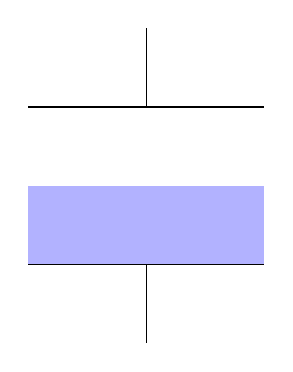
\begin{tikzpicture}
			\def\a{3};
			\def\d{2};

			\begin{scope}
				\draw (-\a/2,0) -- (\a/2,0);
				\draw (-\a/2,\d) -- (\a/2,\d);

				\draw (0,0) -- ++(0,-\d/2);
				\draw (0,\d) -- ++(0,\d/2);
			\end{scope}

			\begin{scope}
				\fill [blue, opacity = 0.3] (-\a/2,0) rectangle (\a/2,\d/2);
			\end{scope}
		\end{tikzpicture}
	\end{figure}
	\begin{figure}[H]
		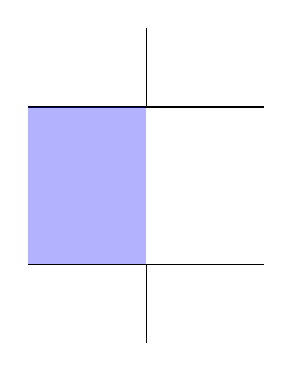
\begin{tikzpicture}
			\def\a{3};
			\def\d{2};

			\begin{scope}
				\draw (-\a/2,0) -- (\a/2,0);
				\draw (-\a/2,\d) -- (\a/2,\d);

				\draw (0,0) -- ++(0,-\d/2);
				\draw (0,\d) -- ++(0,\d/2);
			\end{scope}

			\begin{scope}
				\fill [blue, opacity = 0.3] (-\a/2,0) rectangle (0,\d);
			\end{scope}
		\end{tikzpicture}
	\end{figure}
	Calculate the new capacitance in the two cases.
\end{question}

\begin{solution}
	The arrangements are equivalent to connection of capacitors in series and parallel respectively.
	\begin{figure}[H]
		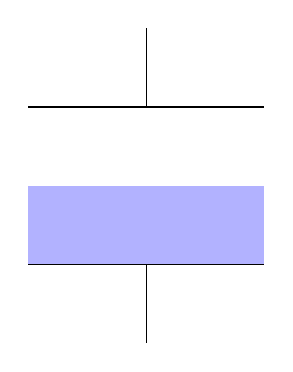
\begin{tikzpicture}
			\def\a{3};
			\def\d{2};

			\begin{scope}
				\draw (-\a/2,0) -- (\a/2,0);
				\draw (-\a/2,\d) -- (\a/2,\d);

				\draw (0,0) -- ++(0,-\d/2);
				\draw (0,\d) -- ++(0,\d/2);
			\end{scope}

			\begin{scope}
				\fill [blue, opacity = 0.3] (-\a/2,0) rectangle (\a/2,\d/2);
			\end{scope}
		\end{tikzpicture}
	\end{figure}
	$\equiv$
	\begin{figure}[H]
		\begin{circuitikz}
			\draw (0,0) to [C = $C_1$] (3,0) to [C = $C_2$] (6,0);
		\end{circuitikz}
	\end{figure}
	In this case,
	\begin{align*}
		C_1 & = \frac{\varepsilon_0 A}{\frac{d}{2}} \\
		C_2 & = \frac{\kappa \varepsilon_0 A}{\frac{d}{2}}
	\end{align*}
	Therefore,
	\begin{align*}
		C_{\textnormal{equivalent}} &= \frac{C_1 C_2}{C_1 + C_2}
	\end{align*}
	~\\
	\begin{figure}[H]
		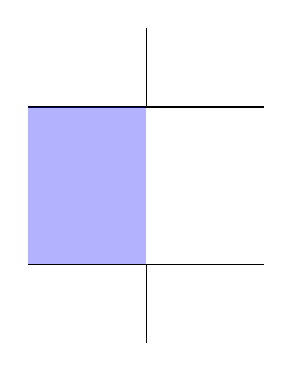
\begin{tikzpicture}
			\def\a{3};
			\def\d{2};

			\begin{scope}
				\draw (-\a/2,0) -- (\a/2,0);
				\draw (-\a/2,\d) -- (\a/2,\d);

				\draw (0,0) -- ++(0,-\d/2);
				\draw (0,\d) -- ++(0,\d/2);
			\end{scope}

			\begin{scope}
				\fill [blue, opacity = 0.3] (-\a/2,0) rectangle (0,\d);
			\end{scope}
		\end{tikzpicture}
	\end{figure}
	$\equiv$
	\begin{figure}[H]
		\begin{circuitikz}
			\draw (0,0) -- (1,0);
			\draw (1,0) to (2,1) to [C = $C_1$] (4,1) to (5,0);
			\draw (1,0) to (2,-1) to [C = $C_2$] (4,-1) to (5,0);
			\draw (5,0) -- (6,0);
		\end{circuitikz}
	\end{figure}
	In this case,
	\begin{align*}
		C_1 & = \frac{\varepsilon_0 \frac{A}{2}}{d} \\
		C_2 & = \frac{\kappa \varepsilon_0 \frac{A}{2}}{d}
	\end{align*}
	Therefore,
	\begin{align*}
		C_{\textnormal{equivalent}} &= C_1 + C_2
	\end{align*}
\end{solution}

\recitation

\begin{question}
	A plate capacitor of area $A$ and distance $d$ is connected to a potential difference $V$.
	A dielectric material of constant $\varepsilon = \kappa_e \varepsilon_0$ is inserted into the capacitor (while connected to the voltage source).
	\begin{enumerate}
		\item Calculate the new capacitance.
		\item How did the free charge on the capacitor plates change in the process?
		\item How did the energy stored in the capacitor change?
	\end{enumerate}
	Now, all the dielectric material is removed.
	Afterward, the capacitor is disconnected from the voltage source.
	A dielectric material of constant $\varepsilon = \kappa_e \varepsilon_0$ is inserted into the capacitor (while disconnected from the voltage source).
	\begin{enumerate}[resume]
		\item Calculate the new capacitance.
		\item How did the potential difference between the plates change?
		\item How did the energy stored in the capacitor change?
	\end{enumerate}
	For both cases, was the dielectric material attracted or repelled by the capacitor?
\end{question}

\begin{solution}
%	Let the capacitance charge, etc\dots
	If there is no dielectric in the capacitor, the capacitance is
	\begin{align*}
		C_0 & = \frac{Q_0}{V_0}                                     \\
                    & = \frac{Q_0}{E_0 d}                                   \\
                    & = \frac{\sigma_0 A}{\frac{\sigma_0}{\varepsilon_0} d} \\
                    & = \frac{\varepsilon_0 A}{d}
	\end{align*}
	\begin{enumerate}[leftmargin = *]
		\item
			After the dielectric material is inserted,
			\begin{align*}
				C_1            & = \frac{Q_1}{V_1}                                              \\
				\intertext{As the battery is connected, the voltage will remain constant. Therefore, $V_0 = V_1$.}
				\therefore C_1 & = \frac{Q_1}{V_0}                                              \\
                                               & = \frac{\sigma_1 A}{\frac{\sigma_1}{\kappa_e \varepsilon_0} d} \\
                                               & = \frac{\kappa_e \varepsilon_0 A}{d}                           \\
                                               & = \kappa_e C_0
			\end{align*}
		\item
			\begin{align*}
				C_1                     & = \frac{Q_1}{V_1}  \\
				\therefore \kappa_e C_0 & = \frac{Q_1}{V_0}  \\
				\therefore Q_1          & = \kappa_e C_0 V_0 \\
                                                        & = \kappa_e Q_0
			\end{align*}
		\item
			\begin{align*}
				U_1 & = \frac{1}{2} C_1 {V_1}^2          \\
                                    & = \frac{1}{2} \kappa_e C_0 {V_0}^2 \\
                                    & = \kappa_e U_0
			\end{align*}
		\item
			\begin{align*}
				C_2            & = \frac{Q_2}{V_2}                                              \\
				\intertext{As the battery is disconnected, the charge cannot flow out and must remain constant. Therefore, $Q_0 = Q_1$.}
				\therefore C_2 & = \frac{Q_0}{V_2}                                              \\
                                               & = \frac{\sigma_2 A}{\frac{\sigma_2}{\kappa_e \varepsilon_0} d} \\
                                               & = \frac{\kappa_e \varepsilon_0 A}{d}                           \\
                                               & = \kappa_e C_0
			\end{align*}
		\item
			\begin{align*}
				C_2                     & = \frac{Q_2}{V_2}          \\
				\therefore \kappa_e C_0 & = \frac{Q_0}{V_2}          \\
				\therefore V_2          & = \frac{Q_0}{\kappa_e C_0} \\
                                                        & = \frac{V_0}{\kappa_e}
			\end{align*}
		\item
			\begin{align*}
				U_2 & = \frac{1}{2} C_2 {V_2}^2                               \\
                                    & = \frac{1}{2} \kappa_e C_0 \frac{{V_0}^2}{{\kappa_e}^2} \\
                                    & = \frac{U_0}{\kappa_e}
			\end{align*}
	\end{enumerate}
	As $U_1 > U_0$, the process of inserting the dielectric increases the potential.
	Therefore, the dielectric is repelled by the plates.\\
	As $U_2 < U_0$, the process of inserting the dielectric decreases the potential.
	Therefore, the dielectric is attracted by the plates.
\end{solution}

\newpage
\part{Electrodynamics}

\begin{question}
	The current and current density are related by the relations
	\begin{align*}
		\overrightarrow{j} & = \rho \overrightarrow{v}   \\
		\overrightarrow{k} & = \sigma \overrightarrow{v} \\
		I                  & = \lambda v
	\end{align*}
	\begin{enumerate}
		\item Calculate the current in a cylinder of radius $R$ carrying uniform charge density $\rho$ moving in velocity $v$ along the cylinder axis.
		\item Calculate the current on a segment of length $L$ in an infinite thin plane carrying uniform charge density $\sigma$ moving in velocity $v$ along the plane surface.
		\item Calculate the current in a thin ring of radius $R$ carrying uniform charge distribution $\lambda$ rotating around its axis with period $T$.
	\end{enumerate}
\end{question}

\begin{solution}
	\begin{enumerate}[leftmargin = *]
		\item
			\begin{align*}
				I & = \iint \overrightarrow{j} \cdot \overrightarrow{\dif A} \\
                                  & = \rho v A
			\end{align*}
		\item
			\begin{align*}
				I & = \int \overrightarrow{k} \cdot \overrightarrow{\dif l} \\
                                  & = \sigma v l
			\end{align*}
		\item
			\begin{align*}
				I & = \lambda v                             \\
                                  & = \lambda \omega R                      \\
                                  & = \lambda \cdot \frac{2 \pi}{T} \cdot R \\
                                  & = \frac{2 \pi \lambda R}{T}
			\end{align*}
	\end{enumerate}
\end{solution}

\begin{question}
	A cylinder of length $L$ and cross-section $A$ is made of metallic material with conductivity $\sigma = \sigma_0 \frac{L}{x}$.
	The bases of the cylinder are connected to potential difference $V$.
	\begin{enumerate}
		\item Calculate the resistivity.
		\item Calculate the current density in the cylinder.
		\item Calculate the electric field inside the metal.
	\end{enumerate}
\end{question}

\begin{solution}
	\begin{enumerate}[leftmargin = *]
		\item
			\begin{align*}
				\sigma          & = \sigma_0 \frac{L}{x} \\
				\therefore \rho & = \frac{1}{\sigma}     \\
                                                & = \frac{x}{\sigma_0 L}
			\end{align*}
		\item
			The cylinder can be considered to be a resistor made up of elemental disk resistors in series.\\
			Consider an elemental disk of thickness $\dif x$ at a distance $x$ from the origin.\\
			Therefore, the resistance of the disk is
			\begin{align*}
				\dif R       & = \frac{\rho \dif x}{A}                             \\
                                             & = \frac{x \dif x}{\sigma_0 L A}                     \\
				\therefore R & = \int\limits_{0}^{L} \frac{x \dif x}{\sigma_0 L A} \\
                                             & = \frac{L^2}{2 \sigma_0 L A}                        \\
                                             & = \frac{L}{2 \sigma_0 A}
			\end{align*}
			Therefore,
			\begin{align*}
				V                      & = I R                      \\
                                                       & = I \frac{L}{2 \sigma_0 A} \\
				\therefore I           & = \frac{2 \sigma_0 A V}{L} \\
				\therefore \frac{I}{A} & = \frac{2 \sigma_0 V}{L}   \\
				\therefore j           & = \frac{2 \sigma_0 V}{L}
			\end{align*}
		\item
			\begin{align*}
				j                                 & = \sigma E \\
				\therefore \frac{2 \sigma_0 V}{L} & = \sigma E \\
				\therefore E                      & = \frac{2 V x}{L^2}
			\end{align*}
	\end{enumerate}
\end{solution}

\addtocounter{question}{1}

\begin{question}
	A cylinder of length $L$ and radius $a$ ($L >> a$) is made of metallic material with resistivity $\rho = \rho_0 \frac{r}{a}$.
	The bases of the cylinder are made of ideal conductor and are connected to potential difference $V$.
	\begin{enumerate}
		\item Calculate the resistance.
		\item Calculate the current in the cylinder.
		\item Calculate the electric field, $\overrightarrow{E}$, inside the metal.
		\item Calculate the current density, $\overrightarrow{j}$, and make sure that $\int \overrightarrow{j} \cdot \overrightarrow{\dif s} = I$.
	\end{enumerate}
\end{question}

\begin{solution}
	\begin{enumerate}[leftmargin = *]
		\item
			The cylinder can be considered to be a resistor made up of elemental cylindrical shell disk resistors in parallel.\\
			Consider an elemental cylindrical shell of radius $r$ thickness $\dif r$.\\
			Therefore, the resistance of the shell is
			\begin{align*}
				\dif R                 & = \frac{\rho L}{2 \pi r \dif r}                       \\
                                                       & = \frac{\rho_0 r L}{2 \pi a r \dif r}                 \\
                                                       & = \frac{\rho_0 L}{2 \pi a \dif r}                     \\
				\therefore \frac{1}{R} & = \int \frac{1}{\dif R}                               \\
                                                       & = \int\limits_{0}^{a} \frac{2 \pi a \dif r}{\rho_0 L} \\
                                                       & = \frac{2 \pi a^2}{\rho_0 L}                          \\
				\therefore R           & = \frac{\rho_0 L}{2 \pi a^2}
			\end{align*}
		\item
			\begin{align*}
				V            & = I R                          \\
				\therefore V & = I \frac{\rho_0 L}{2 \pi a^2} \\
				\therefore I & = \frac{2 \pi a^2 V}{\rho_0 L}
			\end{align*}
		\item
			\begin{align*}
				V            & = E L \\
				\therefore E & = \frac{V}{L}
			\end{align*}
		\item
			\begin{align*}
				j & = \frac{I}{A}                                  \\
                                  & = \frac{\frac{2 \pi a^2 V}{\rho_0 L}}{\pi a^2} \\
                                  & = \frac{2 V}{\rho_0 L}
			\end{align*}
			Therefore,
			\begin{align*}
				\int \overrightarrow{j} \cdot \overrightarrow{\dif s} & = \int\limits_{0}^{a} \frac{2 V}{\rho_0 L} \cdot 2 \pi r \dif r \\
                                                                                      & = \frac{2 \pi a^2 V}{\rho_0 L}                                  \\
                                                                                      & = I
			\end{align*}
			Therefore, $\int \overrightarrow{j} \cdot \overrightarrow{\dif s} = I$.
	\end{enumerate}
\end{solution}

\recitation

\addtocounter{question}{1}

\begin{question}
	A circuit is comprised of a voltage source $(\varepsilon)$, three identical resistors ($R_1 = R_2 = R_3 = R$), a switch ($S$), and an empty capacitor ($C$).
	At $t = 0$ the switch is closed and current starts to flow.
	\begin{figure}[H]
		\begin{circuitikz}
			\draw
				(0,0) to [battery1 = $\varepsilon$] (0,3)
				(0,3) to [R = $R_1$] (3,3)
				(3,3) to [closing switch] (5,3)
				(5,3) to [R = $R_2$] (5,0)
				(5,3) to (7,3)
				(7,3) to [R = $R_3$] (7,1)
				(7,1) to [C = $C$] (7,0)
				(7,0) to (0,0);
		\end{circuitikz}
	\end{figure}
	\begin{enumerate}
		\item Calculate the current flowing in each of the resistors after a very short time ($t \to 0^+$).
		\item Calculate the current flowing in each of the resistors after a very long time ($t \to \infty$).
		\item What is short/long time in this case?
	\end{enumerate}
\end{question}

\begin{solution}
	\begin{figure}[H]
		\begin{circuitikz}
			\draw
				(0,0) to [battery1 = $\varepsilon$] (0,3)
				(0,3) to [R = $R_1$, i = $I_1 + I_2$] (3,3)
				(3,3) to [closing switch] (5,3)
				(5,3) to [R = $R_2$, i = $I_1$] (5,0)
				(5,3) to (7,3)
				(7,3) to [R = $R_3$, i = $I_2$] (7,1)
				(7,1) to [C = $C$] (7,0)
				(7,0) to (0,0);
		\end{circuitikz}
	\end{figure}
	By KVL on the left loop,
	\begin{align*}
		\varepsilon - (I_1 + I_2) R - I_1 R & = 0
	\end{align*}
	By KVL on the larger loop,
	\begin{align*}
		\varepsilon - (I_1 + I_2) R - I_2 R - \frac{Q}{C} & = 0
	\end{align*}
	Therefore, solving,
	\begin{align*}
		3 I_2 R + \frac{2 Q}{C} &= \varepsilon\\
		\therefore 3 R \dod{Q}{t} + \frac{2 Q}{C} &= \varepsilon\\
		\therefore \dod{Q}{t} &= \left( \frac{1}{3 R} \right) \left( \varepsilon - \frac{2 Q}{C} \right)\\
		\therefore \frac{\dif Q}{Q - \frac{C \varepsilon}{2}} &= -\frac{1}{\frac{3 R C}{2}} \dif t\\
		\intertext{Let $\tau = \frac{3 R C}{2}$. Therefore,}
		\therefore \frac{\dif Q}{Q - \frac{C \varepsilon}{2}} &= -\frac{1}{\tau} \dif t\\
		\therefore \int\limits_{-\frac{C \varepsilon}{2}}^{Q - \frac{C \varepsilon}{2}} \frac{\dif Q}{Q - \frac{C \varepsilon}{2}} &= \int\limits_{0}^{t} -\frac{1}{\tau} \dif t\\
		\therefore Q &= \frac{C \varepsilon}{2} \left( 1 - e^{-\frac{t}{\tau}} \right)
	\end{align*}
	Therefore,
	\begin{align*}
		I_2(t) &= \dod{Q}{t}\\
		&= \frac{C \varepsilon}{2} \left( \frac{1}{\tau} \right) e^{-\frac{t}{\tau}}\\
		&= \frac{\varepsilon}{3 R} e^{-\frac{t}{\tau}}
	\end{align*}
	Therefore,
	\begin{align*}
		I_1 &= \frac{\varepsilon - I_2 R}{2 R}\\
		&= \frac{\varepsilon}{2 R} - \frac{I_2}{2}
	\end{align*}
	\begin{enumerate}[leftmargin = *]
		\item
			If $t \to 0^+$,
			\begin{align*}
				I_2 &= \lim\limits_{t \to 0^+} \frac{\varepsilon}{3 R} e^{-\frac{t}{\tau}}\\
				&= \frac{\varepsilon}{3 R} e^0\\
				&= \frac{\varepsilon}{3 R}
			\end{align*}
			Therefore,
			\begin{align*}
				I_1 &= \frac{\varepsilon}{2 R} - \frac{I_2}{2}\\
				&= \frac{\varepsilon}{2 R} - \frac{\frac{\varepsilon}{3 R}}{2}\\
				&= \frac{\varepsilon}{2 R} - \frac{\varepsilon}{6 R}\\
				&= \frac{\varepsilon}{3 R}
			\end{align*}
			Therefore,
			\begin{align*}
				I_0 &= I_1 + I_2\\
				&= \frac{\varepsilon}{3 R} + \frac{\varepsilon}{3 R}\\
				&= \frac{2 \varepsilon}{3 R}
			\end{align*}
		\item
			If $t \to \infty$,
			\begin{align*}
				I_2 &= \lim\limits_{t \to \infty} \frac{\varepsilon}{3 R} e^{-\frac{t}{\tau}}\\
				&= \frac{\varepsilon}{3 R} \cdot 0\\
				&= 0
			\end{align*}
			Therefore,
			\begin{align*}
				I_1 &= \frac{\varepsilon}{2 R} - \frac{I_2}{2}\\
				&= \frac{\varepsilon}{2 R} - 0\\
				&= \frac{\varepsilon}{2 R}
			\end{align*}
			Therefore,
			\begin{align*}
				I_0 &= I_1 + I_2\\
				&= \frac{\varepsilon}{2 R} + 0\\
				&= \frac{\varepsilon}{2 R}
			\end{align*}
		\item
			These short and long times are in comparison to the time constant of the circuit, i.e. $\tau = \frac{3 R C}{2}$.
	\end{enumerate}
\end{solution}

\addtocounter{question}{1}

\newpage
\part{Magnetism}

\section{Lorentz Force}

\begin{question}
	A particle of mass $m$, charge $q$ and velocity $\overrightarrow{v}$ is entering a region of a constant uniform magnetic field $\overrightarrow{B}$.
	The angle between the particle's velocity and the magnetic field is $\theta$.	
	\begin{enumerate}
		\item Describe the trajectory of the particle.
		\item Calculate the cyclotron radius $R$.
		\item Calculate the cyclotron frequency $\omega$ and period $T$.
		\item Calculate the longitudinal distance the particle traverses in one time period.
	\end{enumerate}
\end{question}

\begin{solution}
	\begin{enumerate}
		\item
			The magnetic force acting on the particle is
			\begin{align*}
				\overrightarrow{F} &= q \overrightarrow{v} \times \overrightarrow{B}
			\end{align*}
			Therefore, the force is always perpendicular to the velocity.\\
			Therefore, it changes the direction of the component of the velocity perpendicular to the magnetic field, but not its magnitude.\\
			However the component of the velocity in the direction of $\overrightarrow{B}$ is unaffected by the force.\\
			Therefore, the particle goes in a circle, due to the component of the velocity perpendicular to $\overrightarrow{B}$ and in a straight line due to the component of the velocity parallel to $\overrightarrow{B}$.
			Hence, it goes in a helical path.
		\item
			Let the direction of $\overrightarrow{B}$ be $\hat{k}$.
			\begin{align*}
				\overrightarrow{F} &= q \overrightarrow{v} \times \overrightarrow{B}\\
				\therefore \overrightarrow{F} &= q v \left( \hat{j} \sin \theta + \hat{k} \cos \theta \right) \times \hat{k} B\\
				&= q v B \sin \theta \hat{i}
			\end{align*}
			Therefore,
			\begin{align*}
				\frac{m v^2 \sin^2 \theta}{R} &= q v B \sin \theta\\
				\therefore R &= \frac{m v \sin \theta}{q B}
			\end{align*}
		\item
			\begin{align*}
				\omega &= \frac{v \sin \theta}{R}\\
				&= \frac{v \sin \theta}{\frac{m v \sin \theta}{q B}}\\
				&= \frac{q B}{m}
			\end{align*}
			Therefore,
			\begin{align*}
				T = \frac{2 \pi}{\omega}\\
				&= \frac{2 \pi}{\frac{q B}{m}}\\
				&= \frac{2 \pi m}{q B}
			\end{align*}
		\item
			The component of the velocity in the direction of $\overrightarrow{B}$ is responsible for the longitudinal movement of the particle.\\
			Therefore, the distance traversed by the particle in one time period is,
			\begin{align*}
				d &= v \cos \theta \cdot T\\
				&= v \cos \theta \frac{2 \pi m}{q B}\\
				&= \frac{2 \pi m v \cos \theta}{q B}
			\end{align*}
	\end{enumerate}
\end{solution}

\addtocounter{question}{1}

\section{Biot-Savart Law}

\begin{question}
	Given an arc of radius $R$ and angle $\alpha$, the arc carries current $I$.
	Calculate the magnetic field along the arc's axis.
\end{question}

\begin{solution}
	\begin{align*}
		\dif l &= R \dif \alpha
	\end{align*}
	Let $\overrightarrow{r}$ be the vector joining $\dif l$ and a point at a distance $z$ on the axis.\\
	Therefore,
	\begin{align*}
		\overrightarrow{\dif B} &= \frac{\mu_0}{4 \pi} \frac{I \overrightarrow{\dif l} \times \hat{r}}{r^2}
	\end{align*}
	Therefore, $\overrightarrow{B}$ must be perpendicular to both $\hat{r}$ and $\overrightarrow{\dif l}$.
	\begin{align*}
		\dif B_z &= \frac{\mu_0}{4 \pi} \frac{I \dif l}{r^2} \cos \theta\\
		\therefore B_z &= \frac{\mu_0 I}{4 \pi} \int\limits_{0}^{\alpha} \frac{R \dif \alpha}{r^2} \cos \theta\\
		&= \frac{\mu_0}{4 \pi} \frac{I R^2 \cdot \alpha}{\left( z^2 + R^2 \right)^{\frac{3}{2}}}
	\end{align*}
\end{solution}

\end{document}
